\subsection{Fresh contextual-envelope evaluation}\label{sec:contextresults}
Normal-only selection chooses memory 40; both memories produce zero alarms on the 29,700 M13 development points, and the lower mean width breaks the tie. Each plant uses 9,900 training and 9,900 calibration points. The selected context cutpoints and three widths are Q1 $(0.06969,0.45982)$ and $(0.03599,0.03817,0.04685)$; Q2 $(0.06916,0.45650)$ and $(0.03584,0.04389,0.08261)$; Q3 $(0.06924,0.45714)$ and $(0.05273,0.06456,0.12401)$. Every bin contains at least 102 calibration points, so fallback is unused. Q3's high-context width exceeds tolerance 0.1; the candidate cannot clear in that bin even at zero residual.

All 216 episodes and 2,376 method--episode outcomes complete. Table~\ref{tab:contextfinal} retains all eleven methods. The contextual interval reduces benign points from 42,193 to 332 (99.21\%) and starts from 3,341 to 94 (97.19\%) relative to base dual. Fresh detections rise from 136 to 144. Nevertheless, \textbf{the prospective composite criterion fails}: fresh-detection p95 is 0.731 s versus 0.040 s, exceeding the allowed 0.2 s increase; outside-tolerance inactivity rises from zero to 679/66,357 points (1.023\%); and the joint event count falls from 144 to 62. These three failed cost constraints cannot be replaced by the favorable occupancy result.

\begin{table*}[t]\centering\setlength{\tabcolsep}{4pt}
\caption{Complete fresh synthetic campaign: 72 benign episodes, 424,800 eligible benign points (2.36 h) and 144 attack events. Every method overlaps 144 events, has an observed physical return and is inactive by return + 5 s. Fresh and joint counts use 144; outside inactivity includes detection delay, over 66,357 above-tolerance points. Delays are seconds.}\label{tab:contextfinal}
\begin{tabular}{lrrrrrrrr}\toprule
Method & Benign (\%) & Starts/h & Fresh & Fresh p95 & Outside inactive & Joint & Clear med./p95 & F1\\\midrule
Base dual & 9.932 & 1415.7 & 136 & 0.040 & 0 & 144 & 0.92/1.06 & 0.566 \\
Base no dwell & 1.560 & 2093.6 & 144 & 0.040 & 1 & 143 & 0.59/0.76 & 0.805 \\
RBF dual & 10.156 & 1439.0 & 136 & 0.040 & 0 & 144 & 0.92/1.08 & 0.561 \\
RBF no dwell & 1.620 & 2137.7 & 144 & 0.040 & 1 & 143 & 0.60/0.76 & 0.802 \\
Following point & 1.202 & 1844.9 & 144 & 0.040 & 8,124 & 0 & 0.00/0.00 & 0.902 \\
Tolerance point & 0.104 & 100.8 & 144 & 0.197 & 284 & 40 & 0.00/0.02 & 0.891 \\
Three-of-five & 0.504 & 133.9 & 144 & 0.080 & 256 & 12 & 0.14/0.78 & 0.852 \\
Global interval & 0.072 & 45.8 & 144 & 0.777 & 767 & 62 & 0.06/0.12 & 0.885 \\
Context point & 0.035 & 44.5 & 144 & 0.731 & 1,831 & 0 & 0.00/0.00 & 0.899 \\
Context hysteresis & 0.047 & 44.5 & 144 & 0.731 & 1,016 & 12 & 0.00/0.02 & 0.894 \\
Context interval & 0.078 & 39.8 & 144 & 0.731 & 679 & 62 & 0.06/0.12 & 0.886 \\
\bottomrule\end{tabular}

\end{table*}
\begin{figure*}[t]\centering
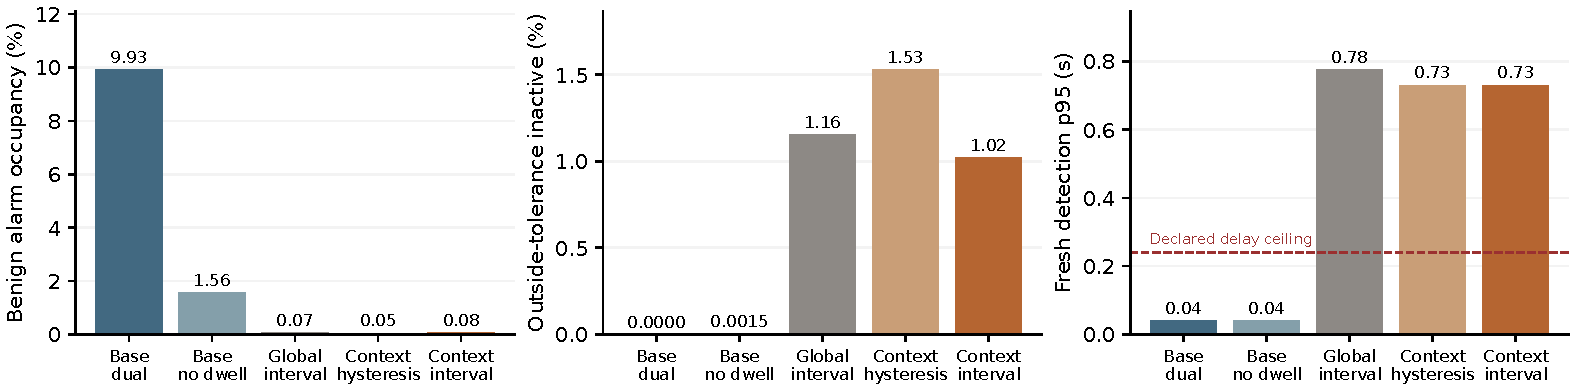
\includegraphics[width=\textwidth]{figures/context_final.pdf}
\caption{Prospectively declared trade-off on new trajectory and plant conditions. The contextual interval reduces benign burden, but increases outside-tolerance inactivity and violates the delay constraint against base dual. Its recovery rule helps relative to matched contextual hysteresis; a constant-width interval achieves the same joint event count. The full roster is retained in Table~\ref{tab:contextfinal}.}\label{fig:contextfinal}
\end{figure*}

The recovery component has a measurable effect within the contextual family: it reduces outside-tolerance inactive points from 1,016 for ordinary hysteresis to 679 and raises joint events from 12 to 62, with identical 144 fresh hits and p95 delay. This comes with 332 rather than 201 benign alarm points, although starts fall from 105 to 94. All declared matched-hysteresis constraints pass. The constant-width interval gives 305 benign points, 108 starts, 767 outside-inactive points and the same 62 joint events. Thus contextual conditioning has a mixed cost profile and does not account for a new dominant method.

Ordinary controls remain informative. The tolerance point rule has 441 benign points and 284 outside-inactive points, with p95 delay 0.197 s; the three-of-five trigger has 2,143 benign points, 256 outside-inactive points and p95 delay 0.080 s. No-dwell variants retain most event support but fragment alarms. Following point attains higher schedule $F_1$ (0.902) while losing 8,124 outside-tolerance points and yielding no joint successes. Missing detections and absent returns happen to be zero in this campaign; favorable conditional clearance still conceals different retention behavior.

A post-evaluation trace decomposition separates the remaining failures: 299 outside-tolerance inactive samples occur before first detection and 380 after it. Of the latter, 321 occur after the first ten-point physical-return interval because distance later crosses tolerance again. Across 39 events with such recrossings, the candidate is inactive on recrossings in 38. Of all 679 inactive-outside samples, 678 lie in the unresolved $L_t\le0.1<U_t$ band and one has incorrect empirical inside evidence. Retaining a previously inactive state through uncertainty is therefore distinct from observing a falling alarm edge outside tolerance. The finite return label is not permanent recovery. This descriptive diagnosis did not select a variant or change the failed criterion.

All 332 benign candidate alarm points occur during authorized changes on perturbed plants. Outside-inactive points are 335 on original plants and 344 on perturbed ones; Lissajous/smoothstep tasks contribute 218/461. The uncertainty band contains 5,636/424,800 benign points (1.327\%); no tested command context exceeds its training maximum. Neither fact validates unseen contexts.

The bounded investigation therefore establishes an additional operating trade-off, not the required original, scientifically justified improvement. Input-dependent thresholds, interval subtraction and hysteresis already exist. Neither these results nor the previous RBF audit establish superiority over CASPER, Kaisar or a complete published robotic monitoring system. The intended contribution remains unresolved; the newly exposed conditions cannot confirm an outcome-informed redesign.
